\documentclass[journal,12pt,two column]{IEEEtran}
\usepackage[cmex10]{amsmath}
\usepackage[utf8]{inputenc}
\usepackage{graphicx}
\usepackage{caption}
\usepackage{subcaption}
\usepackage{stfloats}
\usepackage{amsmath}
\usepackage{amssymb}
\usepackage{amsfonts}
\usepackage{nopageno}
\usepackage[margin=1in]{geometry}
\usepackage{graphicx}
\usepackage{float}
\usepackage{multicol}
\usepackage{hyperref}
\setlength{\parindent}{0em}
\usepackage{color}
\usepackage{comment}

\usepackage[T1]{fontenc}
\setlength{\parindent}{0pt}


\title{AI1103 - Assignment 2}
\author{Monika Kharadi - CS20BTECH11026}
\date{March 2021}
\begin{document}
\maketitle
\section*{\large\textbf{Problem}}
54. Let X be a random variable with the following
cumulative distribution function:\\ \\
F(x) = \begin{cases}
0, & x \textless 0, \\
x^2, & 0\leq x\textless \frac{1}{2} \\
\frac{3}{4}, & \frac{1}{2} \leq x \textless 1 \\
1, & x \geq 1 
\end{cases}\\ \\ 
Then, P( ${\frac{1}{4}}$ $ \textless $ X $\textless $ 1) is equal to. 

\section*{\large\textbf{Solution}}
\begin{align}
 P ( a \textless x \textless b ) =  F(b) - F(a) \end{align}
We want, 
 \begin{align}
S&= P ( {\dfrac{1}{4}}  \textless  X \textless  1)\\
S&= \brac[ F(1) - F(\dfrac{1}{4})]  \\
S&= \brac[ \dfrac{3}{4} - \dfrac{1^2}{4^2}] \\
S&= \dfrac{11}{16}
\end{align}
Hence, P( ${\frac{1}{4}}$ $ \textless $ X $\textless $ 1) is equal to $\frac{11}{16}$

\begin{figure}[H]
\centering
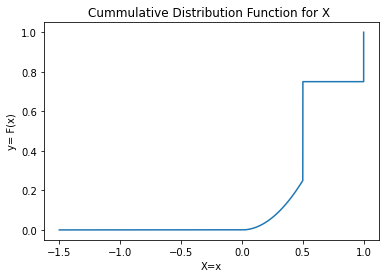
\includegraphics[width=0.5\textwidth]{graph.png}
\label{fig:graph.pmg}
\end{figure}

\end{document}
